% Chapter 1
\chapter{Introdução} % Main chapter title
\label{chap:Introducao} % For referencing the chapter elsewhere

\section{Contextualização}
\label{sec:contextualizacao}

Nos últimos anos, a crescente complexidade dos ambientes laborais, especialmente em setores de alto risco como a indústria, a construção, a energia ou os serviços de emergência, tem aumentado a necessidade de soluções tecnológicas orientadas para a segurança e o bem-estar dos trabalhadores. Nestes contextos, fatores como a fadiga, o stress, a sobrecarga fisiológica e a diminuição da atenção têm um impacto direto no desempenho humano e estão estreitamente relacionados com a ocorrência de acidentes laborais e erros críticos.
Neste quadro, o projeto insere-se na \textbf{Indústria 5.0}, que representa a evolução da Indústria 4.0 para sistemas mais inteligentes, centrados na cooperação entre humanos e máquinas.

\begin{quote}
"A Indústria 5.0 foi proposta para alcançar uma indústria centrada no ser humano, sustentável e resiliente. O enfoque centrado no ser humano coloca os requisitos, preferências e interesses dos trabalhadores no centro do processo de fabrico, passando de um paradigma impulsionado pela tecnologia para um centrado no ser humano e na sociedade." \citeauthor{leng2024} \citeyear{leng2024} \cite{leng2024}.
\end{quote}

A Indústria 5.0 caracteriza-se pela integração de modelos multimodais e o uso de sensores avançados que recolhem dados fisiológicos, de \textbf{dispositivos portáteis} e do ambiente, com o objetivo de oferecer uma previsão cada vez mais precisa e próxima do estado do trabalhador, potenciando a segurança, a eficiência e o bem-estar laboral. Este enfoque procura melhorar a relação humano-máquina, permitindo que as tecnologias não só automatizem processos, mas também colaborem ativamente com os trabalhadores e adaptem o seu funcionamento às suas necessidades e capacidades.

Paralelamente, o avanço dos dispositivos portáteis e sensores biométricos tem permitido a monitorização contínua e não invasiva de variáveis fisiológicas em tempo real. Dispositivos como relógios inteligentes e bandas torácicas possibilitam a aquisição de sinais como a frequência cardíaca, a respiração e a atividade eletrodérmica, gerando grandes volumes de dados durante a jornada laboral. Estes dados constituem uma fonte de informação valiosa para inferir o estado interno do trabalhador e detetar situações de risco antes de se materializarem em incidentes.

Neste contexto, os conceitos de \textbf{gémeos digitais humanos} adquirem uma relevância crescente.

\begin{quote}
"O gémeo digital é uma tecnologia que cria uma réplica digital de uma entidade física mediante o uso de dados em tempo real e modelos computacionais, permitindo que os objetos físicos alcancem maiores níveis de inteligência, automatização e gestão otimizada graças à integração de tecnologias como a Internet das Coisas e a inteligência artificial" \citeauthor{lin2024} \citeyear{lin2024} \cite{lin2024}.
\end{quote}

Um gémeo digital humano permite modelar de forma dinâmica o estado fisiológico de uma pessoa, integrando dados em tempo real com modelos computacionais capazes de interpretar e antecipar a sua evolução. Neste cenário, a \textbf{inteligência artificial} desempenha um papel central, ao facilitar a análise de séries temporais complexas e a extração de padrões não triviais para a deteção e previsão de estados como o stress, a fadiga ou a carga de trabalho.

Neste enquadramento, a presente dissertação insere-se no âmbito do projeto CRIARTE (Construção com Robótica Inteligente e Arquitetura Revolucionária de Tecnologias Emergentes), que visa transformar o setor da construção através da integração de robótica, inteligência artificial e gémeos digitais, promovendo a colaboração segura entre trabalhadores humanos e sistemas autónomos. Em particular, esta dissertação foca-se no eixo do projeto relacionado com a monitorização da saúde e segurança dos trabalhadores, explorando a utilização de dados fisiológicos recolhidos por dispositivos portáteis para a análise e predição de estados associados ao cansaço, stress e fadiga, com vista ao apoio à prevenção de situações potencialmente perigosas em contexto real de obra.

Em resumo, a evolução para ambientes laborais cada vez mais complexos e centrados no ser humano evidencia a necessidade de soluções que permitam monitorizar e interpretar de forma contínua o estado fisiológico dos trabalhadores. A integração de sensores portáteis e modelos de inteligência artificial possibilita antecipar situações de risco e contribuir para a melhoria da segurança e do bem-estar laboral. Neste contexto, os gémeos digitais humanos surgem como uma abordagem integradora para apoiar a prevenção de riscos e a tomada de decisão em cenários laborais complexos.

\section{Descrição do Problema}
\label{sec:problema}

Em ambientes laborais de alto risco (como a construção, a indústria pesada ou os serviços de emergência), o desempenho e a segurança do trabalhador dependem da sua capacidade para manter níveis adequados de energia, atenção e bem-estar físico. O próprio trabalhador muitas vezes não percebe com clareza o seu estado físico (por exemplo, fadiga, stress ou sobrecarga), o que aumenta o risco de acidentes, erros críticos e diminuição do rendimento. Esta situação é especialmente relevante quando o trabalhador interage com outros ativos na obra (outras pessoas, robôs e maquinaria), onde um erro individual pode ter consequências catastróficas, podendo levar mesmo à morte do trabalhador.

Sistemas de monitorização que se centram principalmente em métricas isoladas ou em indicadores estáticos podem ser insuficientes para refletir a complexidade do estado fisiológico do trabalhador e antecipar situações de risco. A variabilidade dos sinais fisiológicos, a influência de fatores externos e as mudanças dinâmicas próprias do ambiente de trabalho fazem com que seja necessário contar com abordagens mais integradas e sofisticadas para a sua análise.

Neste contexto, surge a necessidade de desenvolver modelos computacionais capazes de analisar múltiplos sinais fisiológicos de maneira conjunta ao longo do tempo, assim como sistemas mais avançados, como um gémeo digital humano, que permitam inferir de maneira robusta o estado do trabalhador e apoiar a prevenção de riscos.

O problema central abordado nesta tese consiste em determinar em que medida os modelos de \textbf{aprendizagem automática e aprendizagem profunda} podem ser utilizados para prever estados fisiológicos de trabalhadores em ambientes de alto risco a partir de dados reais obtidos mediante sensores portáteis. Este problema inclui desafios como a seleção e o pré-processamento dos sinais fisiológicos, a segmentação temporal adequada, a escolha de arquiteturas de modelação apropriadas e a avaliação do desempenho dos modelos em cenários próximos da aplicação real. Resolver estes aspetos é essencial para permitir a integração de um módulo preditivo num sistema de gémeo digital humano que contribua de forma efetiva para a prevenção de riscos laborais e para o apoio à tomada de decisões em tempo real.

\section{Objetivos}
\label{sec:objetivos}

Os objetivos desta dissertação são definidos a partir da necessidade de desenvolver uma abordagem capaz de transformar dados fisiológicos recolhidos através de sensores portáteis em informação útil para a monitorização do estado fisiológico e cognitivo de trabalhadores em ambientes laborais de alto risco. Para tal, o trabalho considera de forma integrada as diferentes etapas envolvidas neste processo, desde a caracterização e preparação dos dados até ao desenvolvimento, avaliação e seleção de modelos preditivos, tendo em consideração os requisitos de funcionamento em cenários próximos de tempo real e a sua eventual integração num gémeo digital humano.

\subsection*{Objetivo geral}

O objetivo principal desta tese é desenvolver e avaliar modelos de aprendizagem automática e aprendizagem profunda capazes de prever o estado fisiológico e cognitivo de trabalhadores em ambientes laborais de alto risco, a partir de dados fisiológicos obtidos mediante sensores portáteis, com o fim de contribuir para a segurança e o bem-estar do trabalhador no contexto de um \textbf{gémeo digital humano}.

\subsection*{Objetivos específicos}

Para alcançar o objetivo geral, definem-se os seguintes objetivos específicos. Estes são apresentados na Tabela~\ref{tab:objetivos}, estruturados através de uma abordagem sequencial que associa cada etapa do processo de investigação a uma questão fundamental. Esta organização permite alinhar as necessidades técnicas do projeto (perguntas-chave) com as ações científicas necessárias para a sua resolução (objetivos específicos), garantindo a rastreabilidade e a progressão lógica do trabalho, desde a análise de dados até à integração final no sistema de gémeo digital.

\begin{longtable}{p{3.5cm} p{10.5cm}}
\caption{Objetivos específicos}\label{tab:objetivos}\\
\toprule
\tabhead{perguntas-chave} & \tabhead{objetivos específicos} \\
\midrule
\endfirsthead
\toprule
\tabhead{perguntas-chave} & \tabhead{objetivos específicos} \\
\midrule
\endhead
\endfoot
\bottomrule
\endlastfoot
Que dados tenho? & Analisar e caracterizar os dados fisiológicos recolhidos em ambientes laborais reais, identificando os sinais relevantes e os seus principais padrões temporais. \\
\midrule
Como os preparo? & Desenhar e aplicar técnicas de pré-processamento para sinais fisiológicos, incluindo normalização, filtragem, segmentação temporal e extração de características. \\
\midrule
Que abordagens de modelação exploro? & Explorar diferentes abordagens de modelação para a previsão do estado fisiológico, abrangendo tanto métodos de aprendizagem automática clássica como abordagens de aprendizagem profunda. \\
\midrule
Como se comportam essas abordagens? & Avaliar e comparar as abordagens de modelação consideradas mediante métricas adequadas, analisando a sua capacidade de generalização e a sua viabilidade em cenários próximos a tempo real. \\
\midrule
Qual é viável em tempo real? & Selecionar o modelo ou abordagem mais adequada em função dos resultados obtidos e dos requisitos computacionais do sistema. \\
\midrule
Como o integro no sistema final? & Integrar o modelo preditivo selecionado como um módulo dentro de um sistema de gémeo digital humano, orientado para a monitorização contínua e para a geração de alertas automáticos em contextos laborais de alto risco. \\
\end{longtable}

\subsection*{Discussão e Organização dos Objetivos}

Os objetivos estão organizados para responder a um desafio central: transformar dados fisiológicos gerais em informação útil para acompanhar o estado de cada trabalhador. Para isso, é necessário começar por compreender os dados disponíveis e preparar uma representação adequada, antes de explorar diferentes abordagens de modelação e avaliar a sua capacidade de generalização e a sua compatibilidade com as limitações de uma aplicação próxima do tempo real.

Esta organização reflete, assim, uma sequência metodológica na qual cada etapa fornece a base para a etapa seguinte. A caracterização dos dados permite compreender as suas principais características e limitações; o pré-processamento procura obter uma representação adequada dos sinais; a exploração de diferentes modelos permite analisar diferentes estratégias de previsão; e a avaliação permite determinar não apenas o desempenho preditivo, mas também a sua viabilidade num contexto de utilização contínua. Por fim, a integração no gémeo digital humano procura transformar o modelo desenvolvido num componente funcional de um sistema orientado para a monitorização do trabalhador.

Para além destas etapas, existe uma dificuldade que não é resolvida apenas através da escolha do modelo: o problema de \textit{cold start}, isto é, a dificuldade de produzir previsões úteis quando ainda existem poucos ou nenhuns dados sobre um novo utilizador \cite{schein2002coldstart}. Quando um novo trabalhador começa a utilizar o sistema, a ausência de dados individuais limita a capacidade de caracterizar o seu perfil fisiológico e de produzir previsões personalizadas. Este problema é particularmente relevante num contexto de monitorização contínua, no qual a informação disponível sobre cada trabalhador aumenta progressivamente ao longo do tempo.

Esta questão evidencia que a integração de um modelo preditivo num gémeo digital humano não corresponde apenas à incorporação de um algoritmo de previsão. É também necessário considerar como o sistema inicializa e atualiza o perfil fisiológico individual, como incorpora novos dados e como mantém as previsões ao longo do tempo. Assim, o desenvolvimento dos modelos e a sua integração no sistema devem ser entendidos como partes de um processo contínuo de adaptação às características de cada trabalhador.

Deste modo, os objetivos específicos estabelecem uma cadeia que parte da compreensão dos dados e conduz progressivamente à sua utilização num contexto de aplicação: \textbf{caracterizar, preparar, modelar, avaliar, analisar a viabilidade e integrar}.

\section{Ética e Implicações Sociais na Monitorização Humana}
\label{sec:etica}

A ética no desenvolvimento de tecnologias de monitorização humana vai além do simples funcionamento técnico e relaciona-se diretamente com a responsabilidade para com as pessoas. Ao propor sistemas capazes de recolher sinais biológicos em tempo real, como o ritmo cardíaco ou a temperatura corporal, entra-se num domínio sensível que exige uma base ética sólida. O objetivo principal não deve ser apenas melhorar a eficiência do sistema, mas também proteger o bem-estar do trabalhador e respeitar plenamente a sua dignidade e autonomia.

No contexto industrial e, em particular, na construção civil, a introdução destas tecnologias levanta dúvidas sobre a relação entre a empresa e o trabalhador. Existe o risco de que ferramentas concebidas para melhorar a segurança acabem por ser percecionadas como mecanismos de vigilância ou controlo do desempenho. Esta perceção pode gerar rejeição e desconfiança, dificultando a aceitação do sistema. Por isso, é fundamental que a recolha de dados fisiológicos se limite exclusivamente à proteção da saúde e da segurança, deixando claro que o trabalhador não é um conjunto de números, mas uma pessoa com direito à privacidade.

Outra questão social relevante está relacionada com a equidade e a inclusão. Estas soluções tecnológicas devem ser desenhadas de forma a não excluir determinados trabalhadores, seja por falta de competências digitais ou por diferenças fisiológicas naturais. Um sistema ético deve ser capaz de se adaptar à diversidade humana sem penalizar aqueles que se afastam dos valores considerados “normais”. Além disso, explicar de forma clara que dados são recolhidos, como são utilizados e quem tem acesso à informação é fundamental para gerar confiança entre todos os envolvidos.

Por fim, a cibersegurança e a proteção da informação são aspetos essenciais do ponto de vista ético. Os dados biológicos são particularmente sensíveis e a sua utilização indevida pode ter consequências graves na vida pessoal e profissional dos trabalhadores. Por esta razão, a ética deve orientar o desenho do sistema desde o início, assegurando que a tecnologia atue como um apoio discreto, mas eficaz, sempre orientado para a proteção da segurança física e dos dados pessoais, acima de qualquer interesse técnico ou económico.

\subsection{Enquadramento Legal}
\label{subsec:legal}

Como já foi referido, a necessidade de regulamentar a Inteligência Artificial é crucial, e o Regulamento da Inteligência Artificial da União Europeia (IA Act) \cite{ai_act_2024} representa um marco histórico neste domínio. Este regulamento tem como objetivo impor requisitos e obrigações rigorosos aos fornecedores e desenvolvedores de tecnologias baseadas em IA, garantindo que os sistemas sejam seguros, éticos e fiáveis para os cidadãos europeus. Para tal, o IA Act classifica as utilizações da IA em quatro níveis de risco, tal como ilustrado na Figura~\ref{fig:IAACT}:
\begin{figure}[H]
\centering
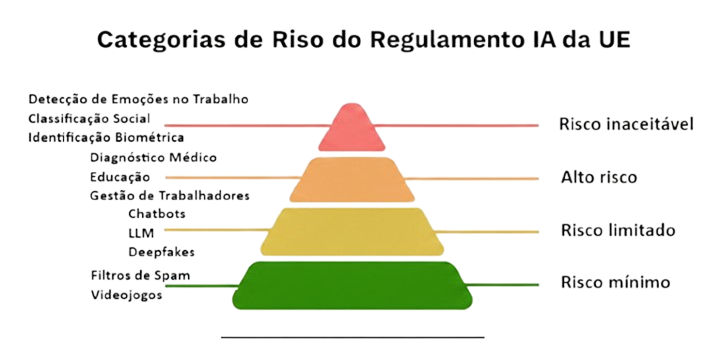
\includegraphics[width=1\textwidth]{ch1/assets/IAACT2.png}
\caption{Pirâmide de Riscos}
\label{fig:IAACT}
\end{figure}

Como se observa na pirâmide de risco, o IA Act organiza os diferentes usos da inteligência artificial de acordo com o nível de risco que podem representar. No topo encontram-se as aplicações de Risco Inaceitável, como a classificação social ou a análise de emoções no local de trabalho, que são proibidas por violarem direitos fundamentais. Abaixo situam-se os sistemas de Alto Risco, que incluem tecnologias críticas para a saúde, as infraestruturas e a gestão de trabalhadores. Seguem-se as aplicações de Risco Limitado, que exigem transparência, como os chatbots ou os conteúdos gerados por IA. Na base encontram-se as aplicações de Risco Mínimo, como os filtros de spam ou os videojogos, que podem ser utilizadas com menos restrições. O regulamento entrou em vigor a 1 de agosto de 2024 \cite{comision_ue_2024}, estabelecendo prazos faseados para a sua aplicação, o que permite às organizações uma adoção responsável e estruturada. O IA Act é o primeiro ato legislativo do mundo focado especificamente na Inteligência Artificial, servindo como referência global, tal como aconteceu com o Regulamento Geral sobre a Proteção de Dados (RGPD) \cite{rgpd_2016}.

O RGPD define normas rigorosas sobre a recolha, o armazenamento e o tratamento de dados pessoais, garantindo a privacidade dos utilizadores. Ao contrário do IA Act, que se centra na lógica do algoritmo, o RGPD refere-se ao tratamento dos dados de todos os residentes na União Europeia, independentemente da localização da organização que utiliza essa informação. No contexto de tecnologias que recorrem a sinais biológicos, o RGPD é particularmente exigente, classificando os dados relativos à saúde como categorias especiais que requerem uma proteção reforçada.

Embora o IA Act e o RGPD demonstrem a preocupação da União Europeia em equilibrar o avanço tecnológico com os direitos das pessoas, estes regulamentos representam apenas um primeiro passo. No setor da construção e da segurança no trabalho, onde os riscos físicos e os acidentes podem ter consequências graves, torna-se necessário dispor de normas claras que permitam desenvolver e utilizar ferramentas inovadoras, como os Gémeos Digitais, sem comprometer a privacidade dos trabalhadores nem os princípios éticos no contexto laboral.

\subsection{Análise Ética e Regulamentar da Solução de Gémeo Digital Humano}
\label{subsec:etica_analise}

A solução proposta nesta dissertação, centrada na monitorização de sinais vitais para a segurança laboral na construção civil, insere-se num ecossistema regulamentar complexo que exige uma análise detalhada. O IA Act, descrito na secção anterior, classifica as aplicações de Inteligência Artificial em função do nível de risco, enquadrando o sistema desenvolvido na categoria de \textbf{Alto Risco}. Esta classificação deve-se ao impacto direto da tecnologia na saúde e segurança dos trabalhadores, bem como à sua utilização no contexto da gestão de recursos humanos.

Ao monitorizar a integridade física em ambientes de alto risco, onde a precisão na deteção de fadiga extrema ou stress é vital, a fiabilidade do sistema torna-se o pilar central da solução. Qualquer falha na análise dos dados fisiológicos poderia ter consequências graves para a vida do trabalhador, o que justifica a exigência de padrões rigorosos de segurança, robustez técnica e cibersegurança. Para cumprir os requisitos de alto risco, o design do Gémeo Digital garante a \textbf{supervisão humana} constante por parte do coordenador de segurança ou do próprio utilizador, assegurando que a tecnologia funcione como um suporte à decisão e nunca de forma autónoma.

Para assegurar a conformidade com o IA Act, destacam-se cinco requisitos de alto risco que são fundamentais e deveriam formar as bases do design da solução: a gestão de riscos (Art.º 9.º) e a governação de dados (Art.º 10.º) para garantir a fiabilidade técnica; a transparência (Art.º 13.º) e a supervisão humana (Art.º 14.º) para permitir o controlo total do utilizador sobre os alertas; e a precisão e cibersegurança (Art.º 15.º) para proteger a integridade da monitorização fisiológica contra falhas ou acessos indevidos.Tendo estes fatores em conta, a solução apresentada procura cumprir todas as regulamentações em vigor e mitigar os desafios éticos associados. 

Relativamente ao RGPD, embora o sistema processe dados biométricos, como o ritmo cardíaco e a temperatura corporal, que pertencem a categorias especiais de dados, o seu design é orientado pelos princípios de privacy by design (a privacidade é integrada desde o início no design do sistema) e minimização de dados (só são recolhidos os dados estritamente necessários). A recolha de informação tem como único objetivo a proteção da vida, garantindo que os dados não sejam utilizados para fins de vigilância intrusiva. No que respeita ao IA Act, a solução afasta-se claramente de práticas classificadas como de Risco Inaceitável, como a inferência de emoções com fins punitivos, mantendo um enfoque estritamente preventivo e fisiológico.

Com supervisão humana e cumprindo os padrões exigidos, esta solução de Gémeo Digital pretende ser um apoio essencial para as equipas de segurança no trabalho. O seu objetivo é criar um ambiente de construção mais seguro e eficiente, combinando a inovação tecnológica com a responsabilidade ética e o respeito total pelos direitos dos trabalhadores.

\section{Estrutura do Documento}
\label{sec:estrutura}

O presente documento está estruturado de forma lógica e sequencial para facilitar a compreensão do problema abordado, da metodologia utilizada e dos resultados obtidos. De seguida, descreve-se brevemente o conteúdo de cada capítulo.

O \hyperref[chap:Introducao]{\textbf{Capítulo 1}}, Introdução, fornece o contexto geral da investigação em ambientes laborais de alto risco e a descrição do problema central. São apresentados os objetivos gerais e específicos, que incluem o desenvolvimento de modelos preditivos e a avaliação de tecnologias emergentes. Adicionalmente, este capítulo aborda as considerações éticas e legais fundamentais no tratamento de dados e no uso de Inteligência Artificial (IA), finalizando com a descrição da estrutura do documento.

O \hyperref[chap:TecnologiasEmergentes]{\textbf{Capítulo 2}}, Revisão Sistemática da Literatura, apresenta a metodologia PRISMA utilizada para realizar uma revisão sistemática da literatura sobre tecnologias emergentes para a monitorização fisiológica e previsão de estados humanos em contextos laborais, incluindo as questões de pesquisa e os resultados obtidos.

O \hyperref[chap:MetodosFerramentas]{\textbf{Capítulo 3}}, Métodos e Ferramentas, explica a abordagem metodológica e os componentes técnicos do sistema. Apresenta a arquitetura do Gémeo Digital Humano, detalhando ferramentas de hardware e software, algoritmos de IA, e o ambiente experimental para recolha e tratamento de dados fisiológicos no contexto laboral.

O \hyperref[chap:Chapter4]{\textbf{Capítulo 4}}, Desenvolvimento e Experimentação, descreve o processo de desenvolvimento técnico e a metodologia experimental para converter dados fisiológicos brutos em indicadores inteligentes do estado humano. Aborda a aquisição, pré-processamento e engenharia de características dos dados, bem como a arquitetura e avaliação dos modelos de aprendizagem automática para classificação de estados dos trabalhadores e suporte à tomada de decisões em tempo real no Gémeo Digital Humano.

O \hyperref[chap:Conclusoes]{\textbf{Capítulo 5}}, Conclusões, sintetiza os principais resultados da investigação e avalia o grau de concretização dos objetivos definidos. Apresenta as contribuições do trabalho, as limitações identificadas e as possibilidades de desenvolvimento futuro, com especial atenção à integração dos modelos num sistema de gémeo digital humano e à sua validação em contextos laborais reais.